\documentclass[12pt]{article} 

\textheight=23.7cm \textwidth=17cm  \topmargin=-1.5cm \hoffset=-2cm

\usepackage[utf8x]{inputenc}
\usepackage[T1]{fontenc}
\usepackage[polish]{babel}
\usepackage{amscd}
\usepackage{amsfonts}
\usepackage{latexsym}
\usepackage{graphicx}
\usepackage{amsthm}
\usepackage{amsmath}
\usepackage{verbatim}
\usepackage{tikz}
\usetikzlibrary{trees,shapes,backgrounds}
\usepackage{multicol}
\usepackage{enumitem}


\def\B{\mathcal{B}}
\def\E{\mathcal{E}}
\def\F{\mathcal{F}}
\def\G{\mathcal{G}}
\def\O{\mathcal{O}}
\def\Q{\mathcal{Q}}
\def\P{\mathcal{P}}
\def\C{\mathcal{C}}
\def\U{\mathcal{U}}
\def\uni{\mathrm{unif}}
\def\Code{\mathrm{Code}}
\def\diag{\mathrm{diag}}
\def\Mah{\mathrm{Mah}}
\def\N{\mathbb{N}}
\def\Z{\mathbb{Z}}
\def\R{\mathbb{R}}
\def\Nor{\mathcal{N}}
\def\I{\mathrm{I}}
\def\f{\mathrm{f}}
\def\m{\mathrm{m}}

\def\C{{\mathbb C}}
\def\Z{{\mathbb Z}}
\def\N{{\mathbb N}}
\def\R{{\mathbb R}}
\def\Q{{\mathbb Q}}

\def\e{\varepsilon}
\def\w{\omega}
\def\dom{\mathrm{dom}}

\includeonly{./tydzien_04/tydzien_04}

\begin{document}

\title{Zadania z Rachunku Prawdopodobieństwa i Statystyki}
\date{}
\maketitle

\section{Tydzień 1}
\medskip
\noindent{\bf Zad. 1} 
\medskip

Rzucamy trzema monetami, możemy rozpisać wszystkie możliwe wyniki, bo nie będzie ich dużo:
$$
\Omega=\{ (O,O,O); (O,O,R); (O,R,O); (R,O,O); (R,R,R); (R,R,O); (R,O,R); (O,R,R);\}
$$
$$
A=\{ (O,O,O); (O,O,R); (O,R,O); (R,O,O)\}
$$
Więc moc obu zbiorów wynosi
$$
|\Omega|=8
$$
$$
|A|=4
$$
Obliczamy prawdopodobieństwo 
$$
P(A)=\frac{|A|}{|\Omega|}=\frac{4}{8}=\frac{1}{2}.
$$
\medskip
\noindent{\bf Zad. 2}
\medskip

Oznaczmy Dame Pik jako "D".
K1-K4 - króle których jest $4$.
J - kolejna dowolna karta.
$$
|A|= |{(D,K1,J), (D,K2,J), (D,K3,J), (D,K4,J)}| = 1 * 4 * 50 = 200
$$

$$
|\Omega| = 51*52*50 = 132600
$$
Obliczamy prawdopodobieństwo
$$
P(A)=\frac{|A|}{|\Omega|}=\frac{200}{132600}=\frac{1}{663}.
$$

\subsection{Zadanie 3}

Z czterech kart: król pik, król karo, dama pik, dama karo losujemy dwie karty. Oblicz prawdopodobieństwo zdarzenia, polegającego
na wylosowaniu jako pierwszej karty jakiegokolwiek króla i jako drugiej karty jakiegokolwiek pika. \\
\\
zdarzenie A - jako pierwszego wylosowano króla pik \\
zdarzenie B - jako pierwszego wylosowano króla karo \\
\[
|A| = 1 , |B| = 1 \cdot 2 = 2 
\]
\[
|\Omega| = 4 \cdot 3 = 12
\]
\[
P(A \cup B) = \frac{1}{12} + \frac{2}{12} = \frac{1}{4}
\]


\subsection{Zadanie 4}

Pierwsza osoba może zająć $10$ różnych miejsc, kolejna $9$ itd aż do osoby $10$ dla której pozostaje tylko jedno miejsce. Ilość możliwych rozsadzeń $10$ osób w $10$ miejscach jest równa iloczynowi możliwości wyboru miejsc każdej kolejnej osoby.
\\
Odp. Możliwych rozsadzeń jest $10 \cdot 9 \cdot . . . \cdot 1 = 10!$


\medskip
\noindent{\bf Zad. 1} 
\medskip

Zakładamy, że talia podana w zadaniu jest talią pokerową i zawiera po cztery karty 9, 10, J, Q, K, A.

Prawdopodobieństwo wyciągnięcia dziesiątki z jednej talii ($|A|=4$, gdyż w talii są cztery 10-tki, $|\Omega|=24$, gdyż losujemy tylko jedną z 24 kart):
$$
P(A)=\frac{|A|}{|\Omega|}=\frac{4}{24}=\frac{1}{6}
$$

Prawdopodobieństwo sukcesu, czyli wyciągnięcia cztery razy dziesiątki z czterech talii:
$$
P(B)=P(A)^4=(\frac{1}{6})^4=\frac{1}{1296}\approx0,077\%
$$

\subsection{Zadanie 6}

$$ |\Omega|= \binom{7}{2}=21 $$

Liczba wystąpień zdarzenia:

$$ |A| = 1* \binom{4}{1}=4 $$

Prawdopodobieństwo zdarzenia:

$$ P(A)=\frac{|A|}{|\Omega|}=\frac{4}{21} $$


\subsection{Zadanie 7}

Wylosowanie nieparzystej liczby oczek dla kostki czworościennej to wylosowanie jednego lub trzech oczek. \\
Zdarzenie A - wylosowanie jednego oczka. Z tabelki 
\[ P(A)=\frac{1}{5} \] \\
Zdarzenie B - wylosowanie trzech oczek. Z tabelki 
\[ P(B)=\frac{1}{15} \] \\
Zdarzenia A i B są rozłączne, więc
 \[ P(A{\cup}B) = P(A) + P(B) = \frac{4}{15} \] \\


\medskip
\noindent{\bf Zad. 8} 
\medskip

Z zadania mamy, że $P(A) = x$, $P(B) = 2x$ i $P(A) \cup P(B) = 1$.
Wiemy też, że zdarzenia $A$ i $B$ wykluczają się. Zatem

\begin{align*}
x + 2x &= 1 \\
3x &= 1 \\
x &= \frac{1}{3}
\end{align*}
\subsection{Zadanie 9}

\begin{itemize}
\item[a)] Ponieważ zdarzenia $A$ i $B$ nie mają częci wspólnej to $P(A \cap B) = 0$
\item[b)]$ P(A \cup B) = P(A) + P(B) + P(A \cap B) = \frac{2}{5} + \frac{1}{5} + 0 = \frac{3}{5}$
\item[c)] $P(A \setminus B) = P(A) - P(A \cap B) = \frac{2}{5} - 0 = \frac{2}{5}$
\end{itemize}


\medskip
\noindent{\bf Zad. 10} 
\medskip

a) Z treści zadania 
$$P({A}\cap{B})=\frac{1}{12}$$
b)$$P({A}\cup{B})=P(A)+P(B)-P({A}\cap{B})$$
Podstawiając dane do wzoru otrzymujemy
$$P({A}\cup{B})=\frac{2}{3}+\frac{1}{5}-\frac{1}{12}=\frac{40}{60}+\frac{12}{60}-\frac{5}{60}=\frac{47}{60}$$
c)$$P({A}\setminus{B})=P(A)-P({A}\cap{B})$$
Wstawiając dane
$$P({A}\setminus{B})=\frac{2}{3}-\frac{1}{12}=\frac{8}{12}-\frac{1}{12}=\frac{7}{12}$$

\textheight=23.7cm \textwidth=17cm  \topmargin=-1.5cm \hoffset=-2cm

\begin{document}


\medskip
\noindent{\bf Zadanie 11} 
\medskip

Spośród 9 klocków wybieramy 4, bez zwracania. Na klockach nie ma cyfry 0 więc nie musimy martwić się możliwością, w której nasza liczba czterocyfrowa zaczynałaby się od zera.

Możliwości losowań:
$$
Cyfry na miejscu dziesiątek tysiecy = 9
$$
$$
Cyfry na miejscu tysiecy = 8
$$
$$
Cyfry na miejscu dziesiątek = 7
$$
$$
Cyfry na miejscu jednostek = 6
$$

$$
9*8*7*6 = 3024
$$

Czyli możemy utworzyć w taki sposób 3024 liczby.

\end{document}

\subsection{Zadanie 12}

Zdefiniujmy omegę - $\Omega = \{\{x,y\} : x, y \in \{1, \dots , 6\}\}$.

$$|\Omega| = 6 * 6 = 36$$

Niech A będzie zdarzeniem, gdzie wypadają różne wyniki na kościach.
Łatwiej będzie policzyć moc zdarzenia przeciwnego - A`.

$$A` = \{\{1,1\}, \{2,2\}, \{3,3\}, \{4,4\}, \{5,5\}, \{6,6\}\}$$
$$|A`| = 6$$

Więc

$$|A| = |\Omega| - |A`| = 36 - 6$$


\subsection{Zadanie 13}

Liter w słowie MATEMATYKA jest $10$, więc wszystkich możliwych ciągów stworzonych z tych liter będzie $10!$
Jednak litery: A, M, T powtarzają się. Dlatego liczba możliwych wyrazów ułożonych z tych liter wynosi
$$
\frac{10!}{2!2!3!}
$$


\medskip
\noindent{\bf Zad. 14} 
\medskip

Rozwiązanie:
Rodzina przy stole musi siedzieć w okreslonej kolejności RDDDR (R-rodzic, D-dziecko).
Możemy ich ustawić na $3!$ (na tyle sposobów dzieci) $* 2!$ (na tyle sposobów rodzice)  $= 12$ sposobów. 
Następnie traktując rodzinę jako jeden element permutujemy ją wraz z pozostałymi osobami siedzącymi przy
stole. Możemy to zrobić na $6!$ sposobów. Wszystkich sposobów rozsadzenia ludzi przy stole jest:
$$
2! * 3! * 6! = 8 640
$$

\subsection{Zadanie 15}

Ze zbioru
\[
 \{1, 2, 3,... ,29, 30\}
\]
 losujemy 10 różnych liczb. Znaleźć prawdopodobieństwa następujących zdarzeń:
 \\
\\a) zdarzenie A = wszystkie wylosowane liczby są nieparzyste
\\
\\ b) zdarzenie B = dokładnie 3 liczby podzielne są przez 5,
\\
\\ c) zdarzenie C = wylosowano 5 liczb parzystych, 5 liczb nieparzystych, w tym dokładnie jedna liczba podzielna przez 10?

\[
n=30,k=10
\]

\[
|\Omega|={n \choose k}={30 \choose 10} = 30045015
\]

\[
|A|={15 \choose 10} = \frac{15!}{5!\cdot10!} = \frac{10 !\cdot 11 \cdot 12 \cdot 13 \cdot 14 \cdot 15}{10! \cdot 125} = 3003
\]

\[
|B|={6 \choose 3} * {24 \choose 7} = \frac{3! \cdot 4 \cdot 5 \cdot 6}{3! \cdot 6} \cdot \frac{17!\cdot18\cdot19\cdot20\cdot21\cdot22\cdot23\cdot24}{17!\cdot7!}= 20 \cdot 346104 = 6 922 080 
\]

\[|C|={15 \choose 5} * {12 \choose 4} * {3 \choose 1} = \frac{10! \cdot 11 \cdot 12 \cdot 13 \cdot 14 \cdot 15}{10! \cdot 5!}  \cdot \frac{8!\cdot9\cdot10\cdot11\cdot12}{8!\cdot4!} \cdot 3= 3003 \cdot 495 \cdot 3 = 29 700\]

Obliczamy prawdopodobieństwa
\[
P(A)=\frac{|A|}{|\Omega|}=\frac{3003}{30045015}=\frac{1}{10005}.
\]

\[
P(B)=\frac{|B|}{|\Omega|}=\frac{ 6 922 080 }{30045015}=\frac{14752}{10 015 005}.
\]
\[
P(C)=\frac{|C|}{|\Omega|}=\frac{ 29 700}{30045015}=\frac{60}{60697}.
\]


\section{Tydzień 2}
\subsection{Zadanie 1}

Niech $(\Omega, F ,P)$ będzie przestrzenią probabilistyczną oraz niech \\ $A,B, A_1,A_2, \ldots, A_n \in F$. Pokazać że:\\ \\

\medskip
\noindent{\bf Podpunkt 1} 
\medskip

Prawdopodobieństwo zdarzenia niemożliwego jest równe zero
$$
P(\emptyset) = 0
$$

Wezmy przykladowa przestrzen $\Omega$ zawierajaca wszystkie mozliwe zdarzenia, ktore zachodza i wezmy przeciwstawne puste zdarzenie $\emptyset$ , ktore nigdy nie zachodzi.


$$ P(\Omega) = 1 \hspace{0.5cm} i \hspace{0.5cm}  P(\emptyset) = 0 $$

Dowod: \\

$$P(\Omega \cup \emptyset) = P(\Omega) + P(\emptyset)$$

Poniewaz $\Omega$ i $\emptyset$ sa wzajemnie sie wykluczajace zatem: 

$$ P(\emptyset) = 0 $$

\medskip
\noindent{\bf Podpunkt 2} 
\medskip


Skończona addytywność. Jeżeli $A_1,A_2, \ldots, A_n$ wykluczają się parami (tj, $A_i \cap A_j = 0$ dla $i \neq j$), to
$$
P\left(\bigcup_{i=1}^{n} A_i \right) = \sum_{i=1}^{n} P(A_i).
$$

$$\sum_{i=1}^{n} P(A_i) = P(A_1) + P(A_2) + \ldots + P(A_n)$$

Poniewaz sa one parami rozlaczne 

$$ P(A_i \cap A_j) = \emptyset , i \neq j$$

\medskip
\noindent{\bf Podpunkt 3} 
\medskip

$$
P(A') = 1 - P(A)
$$\\

Wezmy zdarzenia $A$ i $A'$ takie, ze $P(A \cup A') = \Omega$ i sa one rozlaczne.\\

Stad wiemy, ze:

$$P(A) + P(A') = P(A \cup A') = P(\Omega) = 1$$
Stad:
$$P(A') = 1 - P(A)$$


\medskip
\noindent{\bf Podpunkt 4} 
\medskip

Jeśli $A \subset B$, to 
$$
P(B \setminus A) \leq P(B) - P(A)
$$\\\\


Jesli $A \subset B$ to $ B = A \cup(B \setminus A) $ i $ A \cap (B \setminus A) = \emptyset $ \\
Stad:\\
$$ P(B) = P(A) + P(B \setminus A) $$ 
$$ P(B\setminus A) \geq 0 $$ 

Stad mamy, ze:

$$ P(B) \geq P(A) $$

\medskip
\noindent{\bf Podpunkt 5} 
\medskip

$$
P(A) \leq 1
$$

Zalozmy, ze $\Omega$ jest przestrzenia zawierajaca wszystkie zdarzenia A, wtedy:

$$ P(\Omega) = 1 $$

$$ P(A) \leq P(\Omega) = 1 $$

\medskip
\noindent{\bf Podpunkt 6} 
\medskip


$$
P(A \cup B) = P(A) + P(B) - P(A \cap B)
$$

Wynika z ponizszego diagramu. 

\begin{tikzpicture}[fill=gray]

% left hand
\scope
\clip (-2,-2) rectangle (2,2)
(1,0) circle (1);
\fill (0,0) circle (1);
\endscope
% right hand
\scope
\clip (-2,-2) rectangle (2,2)
(0,0) circle (1);
\fill (1,0) circle (1);
\endscope
% outline
\draw (0,0) circle (1) (0,1)  node [text=black,above] {$A$}
(1,0) circle (1) (1,1)  node [text=black,above] {$B$};

\end{tikzpicture}


\documentclass{article}
\usepackage{mathtools}
\usepackage{polski}
\usepackage[utf8]{inputenc}
\begin{document}


\[ \Omega =\left \{(o,o,o),(o,o,r),(o,r,o),(o,r,r),(r,o,o),(r,o,r),(r,r,o),(r,r,r) \right \} \] 
Prawdopodobieństwo wylosowania trzech reszek pod rząd:

\[ P\left(A\right)= \frac{1}{8} \] 
Prawdopodobieństwo wylosowania nieparzystej ilości reszek:
\[ P\left(B\right)= \frac{4}{8} \] 
Prawdoposobieństwo warunkowe zdarzenia A pod warunkiem zdarzenia B
\[P\left(A|B\right) = \frac{P\left(A \cap B\right)}{P\left( B\right)} = \frac{ P \left(\left \{(r,r,r) \right \} \cap \left \{(o,o,r),(o,r,o),(r,o,o),(r,r,r) \right \}\right)}{ P \left( \left \{(o,o,r),(o,r,o),(r,o,o),(r,r,r) \right \}\right)} = \] 
\[  \frac{\frac{1}{8}}{\frac{4}{8}} = \frac{1}{8} \cdot \frac{8}{4} = \frac{1}{4} \] 

 
\end{document}

\medskip
\noindent{\bf Zad. 3} 
\medskip

C - Chłopiec

D - Dziewczynka

$\Omega = \{(C,D), (C,C), (D,D), (D,C))\}$


\begin{itemize}

\item[a)] starsze dziecko jest chłopcem.
\\$A = \{(C,C)\}$ - rodzina z dwoma chłopcami.
\\B = \{(D,C), (C,C)\} - starsze dziecko jest chłopcem.
\\$A \cap B = \{(C,C)\}$
\\
\\$P(B) = \frac{1}{2}$
\\$P(A \cap B) = \frac{1}{4}$

$$P(A | B) = \frac{P(A \cap B)}{P(B)} = \frac{\frac{1}{4}}{\frac{1}{2}} = \frac{1}{2}$$
\item[b)] jest co najmniej jeden chłopiec.
\\A = \{(C,C)\} - rodzina z dwoma chłopcami.
\\B = \{(C,D), (C,C), (D,C)\} - co najmniej jeden chłopiec.
\\$A \cap B = \{(C,C)\}$
\\
\\$P(B) = \frac{3}{4}$
\\$P(A \cap B) = \frac{1}{4}$

$$P(A | B) = \frac{P(A \cap B)}{P(B)} = \frac{\frac{1}{4}}{\frac{3}{4}} = \frac{1}{3}$$

\end{itemize}

\medskip
\noindent{\bf Zad. 4} 
\medskip

Firma produkuje $98$\% wyrobów odpowiadających normie. Wśród wyrobów spełniających normę jest $75$\% wyrobów pierwszego gatunku. Obliczyć prawdopodobieństwo, że losowo wybrany wyrób jest pierwszego gatunku. \\* \\*		
B - przeszedl norme  98\%  \newline
A - zostal wybrany 1 gatunek \newline
P(A) = ?

$$ P(A|B) = 0,75 $$

$$ P(A|B) = \dfrac{P(A \cap B)}{ P(B)} $$

Stad

$$ 0,75 = \dfrac{P(A \cap B)}{0,98} $$

$$ P(A) = P(A \cap B) = 0,75 * 0, 98 = 0,735 $$

\medskip
\noindent{\bf Zad. 5} 
\medskip

Razem mamy 30 kul - 10 bialych, 20 czarnych.
Prawdopodobienstwo wylosowania 3 kul bialych wynosi:
/begin{center}
  $(10*9*8)/(30*29*28) = (6/203)$
/end{center}

\subsection{Zadanie 6}

Pierwsza urna zawiera 4 białe i jedną czarną kule, druga - 2 białe i 3 czarne.
Losujemy urnę tak, by szansa wybrania pierwszej urny była dwukrotnie mniejsza
niż drugiej. Następnie z wybranej urny losujemy kulę. Jakie jest prawdopodobieństwo
wylosowania kuli białej?\\ 
\\

Rozwiązanie:
$$
P(H_1) \ - \ prawdopodobienstwo \ wyboru \ pierwszej \ urny
$$
$$
P(H_2) \ - \ prawdopodobienstwo \ wyboru \ drugiej \ urny
$$
\\
Z treści zadania wiemy, że:
$$
 P(H_2) = 2* P(H_1)
$$
wiadomo również, że:
$$
 P(H_1) + P(H_2) =1
$$
Rozwiązując układ równań otrzymujemy:
$$
P(H_1) = \frac{1}{3}
$$
$$
P(H_2) = \frac{2}{3}
$$

Podstawiając do wzoru na prawdopodobieństwo całkowite otrzymujemy:
$$
P(A) = P(A|H_1)*P(H_1) + P(A|H_2)*P(H_2) = \frac{4}{5} * \frac{1}{3} + \frac{2}{5} * \frac{2}{3} = \frac{8}{15}
$$
gdzie:
$$
P(A|H_1) \ - \ prawdopodobienstwo \ wylosowania \ bialej \ kuli \ z \ pierwszej \ urny 
$$
$$
P(A|H_2) \ - \ prawdopodobienstwo \ wylosowania \ bialej \ kuli \ z \ drugiej \ urny 
$$
\\


Zadanie można też rozwiązać przy pomocy drzewka. W takim przypadku mnożymy
prawdopodobieństwo wyboru urny przez prawdopodobieństwo wyboru białej kuli z
tej urny. Robimy tak z obiema urnami i wyniki iloczynów sumujemy.

\begin{comment}
$$
\Tree [.Wybor\ urny [.I\\\ urna\\\ $\frac{1}{3}$ [.biała\ $\frac{4}{5}$ ] [.czarna\ $\frac{1}{5}$ ] ]
	 [.II\\\ urna\\\ $\frac{2}{3}$ [.biała\ $\frac{2}{5}$ ]
		 [.czarna\ $\frac{3}{5}$ 
			  ] ] ]
$$
\end{comment}


\subsection{Zadanie 7}

Mamy w urnie b kul białych i c czarnych. Wyciagąmy jedną kulę i natychmiast ją wyrzucamy, nie sprawdzając koloru. Jaka jest szansa wyciągnięcia za drugim razem kuli białej.\\

\noindent
$A_{1}$ - za pierwszym razem wypadła kula biała\\
$A_{2}$ - za pierwszym razem wypadła kula czarna\\
B - za drugim razem wypadła kula biała\\\\
Zatem P(B) = P(B|$A_{1}$)*P($A_{1}$) + P(B|$A_{2}$)*P($A_{2}$)\\\\
Po podstawieniu wartosci:
P(B) = $\dfrac{b}{b+c}*\dfrac{b-1}{b + c - 1} + \dfrac{c}{b+c}*\dfrac{b}{b + c - 1}= \dfrac{b}{b+c}$


\medskip
\noindent{\bf Zad. 8} 
\medskip

Doswiadczenie: Mamy w urnie b kul bialych i c czarnych. Wyciagamy jedna kule i natychmiast ja wyrzucamy, nie sprawdzajac koloru. Nastepnie losujemy kolejna kule. Jakie jest prawdopodobienstwo ze biala jest kula z pierwszego losowania, gdy biala jest kula z drugiego losowania.  
$$
$$
H1 - za pierwszym razem losujemy czarna kule
$$
P(H1) = \frac{c}{b+c}
$$
H2 - za pierwszym razem losujemy biala kule
$$
P(H2) = \frac{b}{b+c}
$$
A -  za drugim razem losujemy kule biala
$$
P(A) = \frac{c}{b+c}*\frac{b}{b+c-1} + \frac{b}{b+c}*\frac{b-1}{b+c-1}
$$
P(H2|A) - prawdopodobienstwo wylosowania kuli bialej w pierwszym losowaniu pod warunkiem ze w drugim zostala wylosowana kula biala.
Z tw Bayesa mamy:
$$
P(H2|A) = \frac{P(A|H2)P(H2)}{P(A)}
$$
a prawdopodobienstwo wylosowania kuli bialej w drugim losowaniu pod warunkiem ze w pierwszym wylosowalismy biala to
$$
P(A|H2) = \frac{b-1}{b+c-1}
$$
czyli
$$
P(H2|A) = \frac{ \frac{b-1}{b+c-1} * \frac{b}{b+c} }{ \frac{c}{b+c}*\frac{b}{b+c-1} + \frac{b}{b+c}*\frac{b-1}{b+c-1} }
$$
po skroceniu otrzymujemy koncowy wynik:
$$
P(H2|A) =\frac{ b^{2} - b} {b^{2} - b + bc}
$$

 \medskip
\noindent{\bf Zad. 9} 
\medskip

W tym zadaniu korzystamy ze wzoru Bayesa:
$$
P(H_j|A)=\frac{P(A|H_j)P(H_j)}{\sum_{i \in I} P(A|H_i)P(H_i) }.
$$
Z zadania 6 mamy wszystkie potrzebne dane, które podstawiamy do powyższego wzoru i otrzymujemy:
$$
P(H_2|A) = \frac{\frac{2}{3}*\frac{2}{5}}{\frac{8}{15}} = \frac{1}{2}
$$

\medskip
\noindent{\bf Zad. 10} 
\medskip

Liczymy prawdopodobienstwo wystapienia defektu w inspekcji:

P(D) = $\frac{2}{10} * \frac{5}{100} + \frac{8}{10} * \frac{3}{10} = \frac{1}{4}$
$$
$$
$$
$$
Liczymy prawdopodobienstwo, ze modul przeszedl proces inspekcji:

P(I/D) = $\frac{P(D/I) * P(I)}{P(D)} = \frac{\frac{5}{100}*\frac{2}{10}}{\frac{1}{4}} = \frac{4}{100}$
$$
$$
$$
$$
 
\tikzstyle{level 1}=[level distance=3.5cm, sibling distance=3.5cm]
\tikzstyle{level 2}=[level distance=3.5cm, sibling distance=2cm]
\tikzstyle{bag} = [text width=4em, text centered]
\tikzstyle{end} = [circle, minimum width=3pt,fill, inner sep=0pt]


\begin{tikzpicture}[grow=right, sloped]




\node[bag] {}
    child {
        node[bag] {I}        
            child {
                node[end, label=right:
                    {D}] {}
                edge from parent
                node[above] {}
                node[below]  {$\frac{5}{100}$}
            }
            child {
                node[end, label=right:
                    {ND}] {}
                edge from parent
                node[above] {}
                node[below]  {$\frac{95}{100}$}
            }
            edge from parent 
            node[above] {}
            node[below]  {$\frac{2}{10}$}
    }
       child {
        node[bag] {NI}        
            child {
                node[end, label=right:
                    {D}] {}
                edge from parent
                node[above] {}
                node[below]  {$\frac{3}{10}$}
            }
            child {
                node[end, label=right:
                    {ND}] {}
                edge from parent
                node[above] {}
                node[below]  {$\frac{7}{10}$}
            }
            edge from parent 
            node[above] {}
            node[below]  {$\frac{8}{10}$}
    };
\end{tikzpicture}

\section{Tydzień 3}
\medskip
\noindent{\bf Zad. 1} 
\medskip

\begin{enumerate}[label=(\alph*)]
\item
$P(A) = \frac{4}{52}  P(B) = \frac{13}{52}$

$P(A \cap B) = \frac{1}{52}$

$P(A \cap B) = P(A) * P(B)$ są niezależne.

\item
$P(A) = \frac{16}{52}  P(B) = \frac{13}{52}$

$P(A) * P(B) = \frac{1}{2} * \frac{13}{52}  P(A \cap B) = \frac{13}{52}$

$P(A \cap B) \neq P(A) * P(B)$ nie są niezależne.
\end{enumerate}
\documentclass{article}
\usepackage[T1]{fontenc}
\usepackage[cp1250]{inputenc}
\usepackage[english,polish]{babel}
\usepackage{polski}
\usepackage{amsmath}
\usepackage{amsfonts}
\begin{document}
\section*{Zadanie 2}
$A=2^n-1$\newline\newline
$B=2^n-2$\newline\newline
$P(A)=\frac{2^n-1}{2^n},\;P(A\cup{B})=\frac{2^n-2}{2^n}$\newline\newline
$P(B)=\frac{2^n-2}{2^n},\;\frac{2^n-2}{2^n}=\frac{2^n-1}{2^n}\cdot{\frac{2^n-2}{2^n}}$\newline\newline
$1=2^n-1$\newline\newline
$n=1$
\end{document}

\subsection{Zadanie 3}

A - odległość losowo wybranego punktu od środka odcinka jest mniejsza niż $\frac{1}{4}$
\[
\Omega=[0, 1]
\]
\[
|\Omega|=1
\]
Zdarzeniu A sprzyjają wszystkie punkty spełniające nierówność
$|x - \frac{1}{2}| < \frac{1}{4}$, więc $x \in(\frac{1}{4}, \frac{3}{4})$, zatem 

\[
A = (\frac{1}{4}, \frac{3}{4})
\]

\[
|A| = |(\frac{1}{4}, \frac{3}{4})| = \frac{1}{2}
\]

\[
P(A) = \frac{1}{2}
\]


\documentclass{article}
\usepackage[utf8]{inputenc}
\usepackage{polski}
\begin{document}
\medskip 
\noindent{\bf Zad. 4}  
\begin{flushleft}
$\Omega$ - zbiór możliwych godzin przybycia dwóch kobiet między 16 a 17\
\\
A - zbiór możliwych godzin przybycia dwóch kobiet tak, aby się spotkały
\[ \Omega =\left \{(a,b) \in <16,17>^2\right \} \]
\[ A = \left \{(a,b) \in <16,17>^2, |a-b| \le \frac{20}{60}\right \} \] 
\[ |a-b| < \frac{20}{60} \Rightarrow a-b \le \frac{20}{60} \wedge a-b \ge -\frac{20}{60}\]
Po przeskalowaniu układu do 0 otrzymujemy rysunek:
\begin{center} \setlength{\unitlength}{0.6mm} \begin{picture}(110,110)
\put(-5,90){\mbox{1}}\put(0,0){\vector(0,0){100}}
\put(90,-5){\mbox{1}}\put(0,0){\vector(1,0){100}} \put(100,-5){\mbox{B}} \put(-5,100){\mbox{A}} 
\qbezier(0,90)(90,90)(90,90)
\qbezier(90,0)(90,90)(90,90)
\qbezier(30,0)(60,30)(90,60)
\qbezier(0,30)(30,60)(60,90)
\qbezier(0,10)(40,10)(40,10)
\qbezier(0,20)(50,20)(50,20)
\qbezier(0,30)(60,30)(60,30)
\qbezier(10,40)(70,40)(70,40)
\qbezier(20,50)(80,50)(80,50)
\qbezier(30,60)(90,60)(90,60)
\qbezier(40,70)(90,70)(90,70)
\qbezier(50,80)(90,80)(90,80)
\put(-25,30){\mbox{a - $\frac{1}{3}$}=b} 
\put(25,-7){\mbox{a + $\frac{1}{3}$}=b} 
\end{picture} \end{center}
Moc $\Omega$ to pole całego kwadratu
\[ \#\Omega = 1\cdot1 \]
Moc A to pole zacznaczonej figury: pole kwadratu - pola trójkątów
\[ \#A = 1 - 2\cdot\frac{1}{2}\cdot\frac{2}{3}\cdot\frac{2}{3}\]
Więc:
\[ P(A) = \frac{1-2\cdot\frac{1}{2}\cdot\frac{2}{3}\cdot\frac{2}{3}}{1} = \frac{5}{9}\]
\end{flushleft}
\end{document}


\medskip
\noindent{\bf Zad. 5} 
\medskip

Zdarzenia $A$ i $B$ są niezależne. Pokaż, że:
\begin{enumerate}
\item Ich dopełnienia też są niezależne.
\item Jeśli $A$ i $B$ są rozłączne, to $P(A) = 0$ lub $P(B) = 0$.
\item Jeśli $A \cup B = \Omega$, to $P(A)=1$ lub $P(B)=1$.
\end{enumerate}

ad. 1)\\

$P(A \cap B) = P(A)*P(B)$

$P(A') = 1-P(A)$

$P(B') = 1-P(B)$

$P(A' \cap B') = P((A \cup B)') = 1-P(A \cup B)=$

 $= 1-[P(A)+P(B)-P(A \cap B)] = 1-P(A)-P(B)+P(A)*P(B)=$

$= 1-P(A)-P(B)*[1-P(A)] = (1-P(A))*(1-P(B)) = P(A')*P(B')$\\

ad. 2)\\

$P(A \cap B) = 0$


$P(A \cap B) = P(A)*P(B)$


$P(A)*P(B) = 0$


$P(A) = 0$ v $P(B) = 0$\\

ad. 3)\\

$1=P(\Omega) = P(A \cup B) = P(A)+P(B)-P(A \cap B) = P(A)+P(B)-P(A)*P(B)$

$P(A)*(1-P(B))+P(B)-1=0$

$[1-P(A)]*[1-P(B)] = 0$

$P(A) = 1$ v $P(B) = 1$


\subsection{Zadanie 6}

Po 10 latach użytkowania $40\%$ komputerów ma problemy z płytami głównymi,
$30\%$ ma problemy z dyskami twardymi, a $15\%$ ma problemy zarówno z jednym
jak i z drugim. Jakie jest prawdopodobieństwo, że $10$-letni komputer będzie
miał wciąż dobrze funkcjonującą zarówno płytę główną, jak i dysk twardy?

\underline{Rozwiązanie:}
$$
$$
$A$ - problem z płytą główną
$$
P(A)=0.4
$$
$B$ - problem z dyskiem twardym
$$
P(B)=0.3
$$
$A \cap B$ - problem zarówno z płytą główną, jak i z dyskiem twardym
$$
P( A \cap B ) = 0.15
$$

$$
1 - P( A \cup B ) = 1 - ( P(A) + P(B) - P( A \cap B ) ) = 
$$
$$
= 1 - P(A) - P(B) + P( A \cap B ) = 1 - 0.4 - 0.3 + 0.15 = 0.45
$$

\underline{Odpowiedź:}

Prawdopodobieństwo, że $10$-letni komputer będzie miał wciąż dobrze funkcjonującą
płytę główną oraz dysk twardy wynosi $45\%$.


\medskip
\noindent{\bf Zad. 7} 
\medskip
Z kwadratu jednostkowego wybrano losowo punkt o współrzędnych (x,y). Wyznaczyć:
$$
1. \ P(min(x,y) <a)
$$
$$
2 \ P(max(x,y) < a)
$$
$$
3. \ P(|x-y| < a)
$$
$$
4. \ P(\frac{1}{2}(x+y) < a)
$$
1)
$$
P(min(x,y) <a) =  2a-a^2
$$
2)
$$
P(max(x,y) < a) = a^2
$$
3)

$$
-a<|x-y|<a
$$
$$
y = x-a  \  \  \  \  \  \  \  \  \ y = x+ a
$$
$$
 P(|x-y| < a)  = 1 - (1-a)^2
$$
4)
$$
y < 2a -x
$$
$$
a = \frac{1}{2} \longrightarrow P(A) = \frac{1}{2}
$$
$$
a < \frac{1}{2} \longrightarrow P(A) = \frac{1}{2} * 2a *2a
$$
$$
a > \frac{1}{2} \longrightarrow P(A) = 1 - \frac{1}{2} (1-2a)^2
$$

\medskip
\noindent{\bf Zad. 8} 
\medskip
\\

\begin{flushleft}
$\Omega$ - zbiór możliwych godzin w których procesy zgłaszają się po zasób\
\\
A - zbiór możliwych godzin awarii systemu
\[ \Omega =\left \{(a,b) \in <10,12>^2\right \} \]
\[ A = \left \{(a,b) \in <10,12>^2, |a-b| \le \frac{10}{120}\right \} \] 
\[ |a-b| < \frac{10}{120} \Rightarrow a-b \le \frac{10}{120} \wedge a-b \ge -\frac{10}{120}\]
Po przeskalowaniu układu otrzymujemy rysunek:
\begin{center} \setlength{\unitlength}{0.6mm} 
	\begin{picture}(110,110)
	
	\put(-5,90){\mbox{1}}\put(0,0){\vector(0,0){100}}
	\put(90,-5){\mbox{1}}\put(0,0){\vector(1,0){100}} 
	
	\put(100,-5){\mbox{b}} 
	\put(-5,100){\mbox{a}} 
	
	\qbezier(0,90)(90,90)(90,90)
	\qbezier(90,0)(90,90)(90,90)
	
	\put(0,10){\line(1,1){80}}
	\put(10,0){\line(1,1){80}}
	
	\put(0,10){\line(1,0){20}}
	\put(10,20){\line(1,0){20}}
	\put(20,30){\line(1,0){20}}
	\put(30,40){\line(1,0){20}}
	\put(40,50){\line(1,0){20}}
	\put(50,60){\line(1,0){20}}
	\put(60,70){\line(1,0){20}}
	\put(70,80){\line(1,0){20}}
	
	\put(-25,30){\mbox{a - $\frac{1}{12}$}=b} 
	\put(25,-7){\mbox{a + $\frac{1}{12}$}=b} 

	\end{picture} 
\end{center}
Moc $\Omega$ to pole całego kwadratu
\[ \#\Omega = 1\cdot1 \]
Moc A to pole zacznaczonej figury: pole kwadratu - pola trójkątów
\[ \#A = 1 - 2\cdot\frac{1}{2}\cdot(\frac{11}{12})^2 = 1 - \frac{121}{144} = \frac{23}{144}\]
Więc:
\[ P(A) = \frac{23}{144} \]
\end{flushleft}

\medskip 
\noindent{\bf Zad. 9}  
\medskip

Dane są zdarzenia niezależne $A$ i $B$ przy czym $P(A) = P(B) = p$. Jak jest szansa, że zaszły oba, jeśli wiadomo, że zaszło co najmniej jedno.

$$
P(A \cap B | A \cup B ) =  \frac {P(A \cap B ) \cap P ( A \cup B)} { P ( A \cup B)} = 
\frac {P(A \cap B )} { P ( A \cup B)} =  
\frac {P(A) * P (B)} {P(A) + P (B) - P ( A \cap B)} = 
$$
$$
\frac {p * p} {p + p - p * p} = \frac {p ^ {2} }{2p - p ^{2}} = 
\frac {p ^{2}} {p( 2 - p) } = 
\frac {p} { 2 - p } 
$$

\medskip
\noindent{\bf Zad. 10} 
\medskip

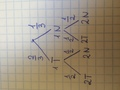
\includegraphics{./tydzien_03/zad_10.jpg}

$P(A) = \frac{\frac{2}{8}\frac{1}{2}}{\frac{2}{3}\frac{1}{2} + \frac{1}{8}\frac{1}{2}}
 = \frac{\frac{1}{3}}{\frac{1}{3} + \frac{1}{6}} = \frac{2}{3}i$


\begin{zad}
System może być zainfekowany przez spyware albo drogą internetową albo przez e-mail. Przez 70 procent czasu spyware nadchodzi drogą internetową, przez 30 procent - drogą mailową. Jeśli przychodzi drogą internetową, system wykrywa go natychmiast z prawdopodobieństwem 0.6. Jeśli przez e-mail -- z prawdopodobieństwem 0.8. Przez jaki procent czasu spyware jest wykrywany? Odp: 0.66 \\

\underline{Dane:}
$$
$$
$H_{1}$ - spyware nadszedł drogą internetową
$$
P(H_{1}) = \frac{7}{10}
$$
$H_{2}$ - spyware  nadszedł przez e-mail
$$
P(H_{2}) = \frac{3}{10}
$$
$A$ -  spyware został wykryty
$$
P(A|H_{1}) = \frac{6}{10}
$$
$$
P(A|H_{2}) = \frac{8}{10}
$$

\underline{Rozwiązanie:}\\
$$
P(A) = P(A|H_{1}) \cdot P(H_{1}) + P(A|H_{2}) \cdot P(H_{2}) = 
$$
$$
= \frac{7}{10} \cdot  \frac{6}{10} + \frac{3}{10} \cdot \frac{8}{10} = 0.42 + 0.24 = 0.66
$$

\underline{Odpowiedź:} \\
Spyware jest wykrywany przez $66\%$ czasu.
\end{zad}

\subsection{Zadanie 12}

Program składa się z 2 bloków napisanych niezależnie przez 2 programistów. Pierwszy zawiera usterkę z prawdopodobieństwem 0.2, drugi -- z prawdopodobieństwem 0.3. Jeśli program zwróci błąd, jakie jest prawdopodobieństwo, że oba moduły zawierają usterkę? Odp: 0.1364

Rozwiązanie
$$
\Omega=\  0,2 * 0,3 + 0,8 * 0,3 + 0,2 * 0,7
$$

$$
|\Omega|=0,44
$$

A - Oba moduły zawierają usterke

$$
|A|=0,2 * 0,3 = 0,06
$$

$$
P(A)=\frac{|A|}{|\Omega|}=\frac{0,06}{0,44}. = 0,1364
$$


\subsection{Zadanie 13}

$W$ - wystąpiła awaria\\
$P(A) = 0,2$\\
$P(B) = 0,4$ \\
$P(A \cap B) = P(A)P(B) = 0,2 \cdot 0,4 = 0,08$\\
$P(A \setminus B) = 0,2 - 0,08 = 0,12$\\
$P(B \setminus A) = 0,4 - 0,08 = 0,32$\\
$P(W | A \setminus B) = 0,5$\\
$P(W | B \setminus A) = 0,8$\\
$P(W | A \cap B) = 0,9$\\
z twierdzenia Bayesa:\\
$P(A \cap B | W) = \frac{P(W | A \cap B) \cdot P(A \cap B)}{P(W)}= \frac{P(W | A \cap B) \cdot P(A \cap B)}{P(W | A \setminus B) \cdot P(A \setminus B) + P(W | B \setminus A) \cdot P(B \setminus A)+ P(W | A \cap B) \cdot P(A \cap B)} = \frac{0,9 \cdot 0,08}{0,5 \cdot 0,12 + 0,8 \cdot 0,32+ 0,9 \cdot 0,08}=$\\
$=\frac{0,072}{0,388} \approx 0,19$


\subsection{Zadanie 14}

$P(A) = 0,1$, $P(B) = 0,2$, $P(C) = 0,3$, $P(D) = 0,4$, $P(E) = 0,5$ 

1.
$P(I) = 1 - P ( \overline{A} \cap \overline{B} \cap \overline{C}
\cap \overline{D} \cap \overline{E}) = 1 - ( 0,9 \cdot 0,8 \cdot 0,7
\cdot 0,6 \cdot 0,5=)\\= 1 - 0,1512 = 0,8488$

2.

$P(II) = 1 - ( P(\overline{I}) + 
P(A \cap \overline{B} \cap \overline{C}\cap \overline{D} \cap \overline{E}) +
P(B \cap \overline{A} \cap \overline{C}\cap \overline{D} \cap \overline{E}) +\\
+P(C \cap \overline{A} \cap \overline{B}\cap \overline{D} \cap \overline{E}) +
P(D \cap \overline{A} \cap \overline{B}\cap \overline{C} \cap \overline{E}) +
P(E \cap \overline{A} \cap \overline{B}\cap \overline{C} \cap \overline{D}) )=\\
= 1 - ( 0,1512 + 0,1512+0,1008+0,0648+0,0378+0,0168) = 1 - 0,5226 =\\= 0,4774
$\\

3.

$P(III) = P(A \cap B \cap C \cap D \cap E) = 0,1 \cdot 0,2 \cdot 0,3 \cdot 0,4 \cdot 0,5 = 0,0012
$


1.\\
$$
|A| = {6\choose2}\\
|\Omega| = {10\choose 6}\\
P(A) = \frac{{6\choose2}}{{10\choose 6}} = \frac{\frac{6!}{2!(6-2)!}}{\frac{10!}{6!(10-6)!}}
= \frac{6!}{2!4!}\cdot\frac{6!4!}{10!} = \frac{3\cdot4\cdot5\cdot6}{1}\cdot\frac{1}{7\cdot8\cdot9\cdot10}=\\
=\frac{1\cdot1\cdot1\cdot6}{7\cdot2\cdot3\cdot2}=\frac{1}{7\cdot2}=\frac{1}{14}\approx7,143\%
\\
$$
\\2\\
$$
|B|={6\choose2}\\
$$

$$
|\Omega|={6\choose2}+{6\choose3}+{6\choose4}+{6\choose5}\\

P(B) = \frac{{6\choose2}}{{6\choose2}+{6\choose3}+{6\choose4}+{6\choose5}}=
\frac{\frac{5\cdot6}{2}}{\frac{6!}{2!4!}+\frac{6!}{3!3!}+\frac{6!}{4!2!}+\frac{6!}{5!}}=\\
\frac{15}{15+\frac{4\cdot5\cdot6}{2\cdot3}+15+6}
=\frac{15}{36+20}=\frac{15}{56}\approx26,786\%
$$


\subsection{Zadanie 1}

\begin{enumerate}[label=(\alph*)]
\item $X=\{0,1\}$
\item $X=\{1,2,\dots,52\}$
\item $X=\{1,2,3,4,5,6\}$
\item $X=\{0,1\}$
\end{enumerate}

\subsection{Zadanie 2}

$X ~ Bin(n, p)$; $n$ - ilość prób, $p$ - prawdopodobieństwo wygranej
\begin{enumerate}[label=(\alph*)]
\item
$$ k = 2, X ~ Bin(n = 4, p = \cfrac{1}{2}) $$
$$
P(X = 2) * {{4}\choose{2}} * {{1}\choose{2}}^2 * {{1}\choose{2}}^2 = 6 * \cfrac{1}{4} * \cfrac{1}{4} = \cfrac{3}{8}
$$

\item
$$ k = 3, X ~ Bin(n = 6, p = \cfrac{1}{6}) $$
$$
P(X = 3) = {{6}\choose{3}} * {{1}\choose{2}}^2 * {{1}\choose{2}}^2 = 20 * \cfrac{1}{8} * \cfrac{1}{8} = \cfrac{5}{16}
$$
\end{enumerate}

$$Ex = n * p$$
$$Var X = n * p(1 - p)$$

\begin{enumerate}[label=(\alph*)]
\item
$$ Ex = 4 * \cfrac{1}{2} = 2 $$
$$ Var X = 2 * \cfrac{1}{2} = 1 $$

\item
$$ Ex = 6 * \cfrac{1}{2} = 3$$
$$Var X = 3 * \cfrac{1}{2} = \cfrac{3}{2}$$
\end{enumerate}

\subsection{Zadanie 3}

Firma zakupiła $4$ nowe monitory tej samej marki. Prawdopodobieństwo, że monitor tej
marki ulegnie awarii w okresie gwarancji wynosi $0,05$. Oblicz prawdopodobieństwo, że

\begin{enumerate}[label=(\alph*)]
\item dwa monitory ulegną awarii w okresie gwarancji

$$
P(X=2) = \frac{4}{2} * 0.05^{2}* 0.95^{2}
$$

\item nie wszystkie monitory ulegną awarii w okresie gwarancji
$$
P(X<4)=1-P(X=4)=1- \frac{4}{4} * 0.05^{4} * 0.05^{0}
$$


\item co najmniej jeden monitor ulegnie awarii w okresie gwarancji
$$
P(X>0)=1- P(X=0)=1- \frac{4}{0} * {0.05}^0 * {0.35}^4
$$
\end{enumerate}

Czy te zdarzenia można opisać za pomocą jednej zmiennej losowej czy potrzebujemy różnych? 
Policz dla wyznaczonych zamiennych losowych wartość oczekiwaną i wariancję.

$$ 
EX=4*{0.05}
$$

$$
Var(X)=4*{0.05}*{0.95}
$$

\subsection{Zadanie 4}

\begin{enumerate}[label=(\alph*)]
\item
$$
A - wypadł orzeł
$$
P(A)=\frac{1}{2}
$$
Zmienna ma rozkład geometryczny. Wzór na prawdopodobieństwo:
$$
P(X=k)=(1-p)^{(k-1)}p
$$
k=4
$$
P(X=4)=(1-\frac{1}{2})^{(4-1)}\frac{1}{2} = (\frac{1}{2})^3 \frac{1}{2} = \frac{1}{16}
$$
\item
$$
E(X) = \frac{1}{p}
$$
E(X) = \frac{1}{\frac{1}{2}} = 2
$$
Var(X) = \frac{1-p}{p^2}
$$
Var(X) = \frac{1-\frac{1}{2}}{(\frac{1}{2})^2} = 2
$$
\end{enumerate}

\subsection{Zadanie 5}

\begin{enumerate}[label=(\alph*)]
\item
Liczba spółek dostępnych na giełdzie: $N=20$
Liczba spółek, których kurs wzrósł: $M=14$
Liczba spółek, które zakupił inwestor: $n=8$

\item Prawdopodobieństwo, że wśród zakupionych przez inwestora akcji,
kurs co najmniej siedmiu wzrósł (zmienna losowa o rozkładzie hipergeometrycznym):

\begin{align*}
P(X \geq 7)=P(X=7)+P(X=8) &= \\
\frac{\binom{14}{7}* \binom{20-14}{8-7}}{\binom{20}{8}}+\frac{\binom{14}{8}* \binom{20-14}{8-8}}{\binom{20}{8}} &= \\
\frac{\binom{14}{7}*\binom{6}{1}+\binom{14}{8}*\binom{6}{0}}{\binom{20}{8}} &= \\
\frac{\frac{14!}{7!*7!}*\frac{6!}{1!*5!}+\frac{14!}{8!*6!}*\frac{6!}{0!*6!}}{\frac{20!}{8!*12!}} &= \\
\frac{\frac{7!*8*9*10*11*12*13*14}{7!*2*3*4*5*6*7}*\frac{5!*6}{5!}+\frac{8!*9*10*11*12*13*14}{8!*2*3*4*5*6}*\frac{6!}{6!}}{\frac{12!*13*14*15*16*17*18*19*20}{12!*2*3*4*5*6*7*8}} &= \\
\frac{20592+3003}{125970} &=
\frac{23595}{125970}\approx 0.1873
\end{align*}

\end{enumerate}

\subsection{Zadanie 6}

W klasie jest 20 osób przy czym dziewczyn jest o 6 więcej niż chłopców.
Nauczyciel wybiera losowo do odpowiedzi cztery osoby, przy czym osoba raz
wybrana nie jest pytania ponownie. Oblicz prawdopodobieństwo, że nauczyciel
wybierze:

\begin{enumerate}
\item samych chłopców
\item tyle samo dziewcząt co chłopców
\end{enumerate}

$N$ - liczba osób w klasie, $N = 20$
$n$ - liczba osób pytanych, $n = 4$
$M$ - liczba chłopców, $M = 7$

Rozkład prawdopodobieństwa zmiennej losowej X o rozkładzie hipergeometrycznym
wyraża się wzorem:

$$P(X=k) = \dfrac{\binom{M}{k} * \binom{N-M}{n-k}}{\binom{N}{n}}$$

\begin{enumerate}
\item
$P(X=4)= \dfrac{\binom{7}{4} * \binom{13}{0}}{\binom{20}{4}}$

\item
Trzeba wybrać dwóch chłopaków z 7 i resztę osób z grupy dziewczyn

$A$ - zdarzenie w którym nauczyciel wybrał dwóch chłopców i dwie dziewczynki

$P(A) = P(X=2)= \dfrac{\binom{7}{2} * \binom{13}{2}}{\binom{20}{4}}$
\end{enumerate}
\subsection{Zadanie 7}

\begin{enumerate}[label=(\alph*)]
\item
$$
P(X=0) = e^{-2,4}*\frac{2,4^{0}}{0!}=e^{-2,4}
$$

$$
P(X=1)= e^{-2,4}*\frac{2,4^{1}}{1!}=e^{-2,4}*2,4
$$
$$ 
EX=2,4
$$
$$
Var(X)=2,4
$$

\item Żeby policzyć prawdopodobieństwo, że zmienna losowa będzie
miała wartość powyżej 5 można policzyć prawdopodobieństwo zdarzenia
przeciwnego.

$$
P(X>5)=1-P(X=0)-P(X=1)-P(X=2)-P(X=3)-P(X=4)-P(X=5)
$$

$$
P(X>5)= e^{-2,4}
-e^{-2,4}*2,4 
-\frac{e^{-2,4}*2,4^{2}}{2}- 
\frac{e^{-2,4}*2,4^{3}}{6}-
\frac{e^{-2,4}*2,4^{4}}{24}-
\frac{e^{-2,4}*2,4^{5}}{120}
$$

Zmienna losowa o rozkładzie Poissona opisuje zmienne, w których zdarzenia występują rzadko.
\end{enumerate}

\subsection{Zadanie 8}

\begin{enumerate}[label=(\alph*)]
\item
$$
\chi_{[2,6]}(x) = \left\{ \begin{array}{ll}
\frac{1}{4} & \textrm{gdy $x \in [2,6]$}\\
0 & \textrm{gdy $x \notin [2,6]$}
\end{array} \right.
$$
\item
$$
P(X \in [3, 3.5]) = \int\limits_{3}^{3.5} \frac{1}{4} dx = \frac{1}{4}\cdot (3.5 - 3) = \frac{1}{4}\cdot \frac{1}{2} = \frac{1}{8}
$$
\item
$$
P(X \in (3, 3.5)) = P(X \in [3, 3.5]) = \frac{1}{8}
$$
\end{enumerate}

\subsection{Zadanie 9}


Gęstość zmiennej losowej $X$ o rozkładzie wykładniczym z parametrem $\lambda$ jest dana przez 
$$
f(x) = \left\{ \begin{array}{ll}
\lambda \cdot e^{-\lambda x} & \textrm{gdy $x > 0$}\\
0 & \textrm{gdy $x \leq 0$}
\end{array} \right.
$$

Zatem jeżeli za parametr  $\lambda$  przyjmiemy 1 otrzymamy:

$$
f(x) = \left\{ \begin{array}{ll}
 e^{- x} & \textrm{gdy $x > 0$}\\
0 & \textrm{gdy $x \leq 0$}
\end{array} \right.
$$
  
Co przedstawione zostało na rysunku. Prawdopodobieństwo, że  $X \in [0,1]$ zostało przedstawione na rysunku poprzez obszar zakreskowany na czerwono.

Obliczmy prawdopodobienstwo zdarzenia że $X \in [0,1]$:

$$
\int_{0}^{1} e^{- x} dx = [-e^x]_{0}^{1} = -e^{-1} + 1
$$

\subsection{Zadanie 10}
$$P(X>0)=\int\limits_{0}^{\infty}f(x)dx=\frac{1}{2}$$

Wykres tej funkcji jest parzysty a pole całego wykresu wynosi 1 
więc z połowy jest $\frac{1}{2}$.
\subsection{Zadanie 11}
\begin{enumerate}[label=(\alph*)]
\item

\begin{align*}
E(X) &= \frac{1}{\lambda}\\
&= \frac{1}{\frac{1}{5}} * 3\\
&= \frac{3}{\frac{1}{5}}\\
&= 3 * 5\\
E(X) &= 15
\end{align*}


\begin{align*}
Var(X) &= \frac{1}{\lambda^2}\\
&= \frac{1}{(\frac{1}{5})^2} * 3 \\
&= \frac{1}{\frac{1}{25}} \\
&= 25 * 3 \\
&= 75
\end{align*}

\item Korzystając z formuły Gamma-Poissona
$$
P(T<t) = P(X \geq \alpha), \; \; \; \; \; \; (Bo: P(T<t) = P(T \leq t))
$$

gdzie $$x = 3, \alpha = \frac{1}{5}, t=12 \;\;\;\; (x=3 \,\,\, \text{bo mamy 3 bloki})
$$
$$
P(X \geq 3) = 1 - P(0) - P(1) - P(2) = 1 - F(2)
$$
$$
P(T < 12) = P(X \geq 3) = 1 - F(2) = 1 - 0.597
$$
$$
= 0.430
$$

$\Rightarrow$ Prawdopodobieństwo, że cały proces kompilacji zostanie przeprowadzony w czasie mniejsyzm niż 12 minut, wynosi $\approx 43 \%$

\end{enumerate}

\subsection{Zadanie 12}

Pięć procent częsci komputerowych produkowanych przez pewnego producenta jest wadliwych. Jakie jest prawdopodobieństwo, że próba 16 częsci zawiera więcej niż 3 częsci wadliwe?

$$
P(X = 0)={16\choose 0}*(0,95)^{16}*(0,05)^{16-16}=(0,95)^{16}
$$
$$
P(X = 1)={16\choose 1}*(0,95)^{15}*(0,05)^{16-15}=16*(0,95)^{15}*(0,05)
$$
$$
P(X = 2)={16\choose 2}*(0,95)^{14}*(0,05)^{16-14}=120*(0,95)^{14}*(0,05)^{2}
$$
$$
P(X = 3)={16\choose 3}*(0,95)^{13}*(0,05)^{16-13}=560*(0,95)^{13}*(0,05)^{3}
$$

$$
P(X > 3)=1-[P(X = 0) + P(X = 1) + P(X = 2) + P(X = 3)]
$$

\subsection{Zadanie 13}
Niech $X$ będzie zmienną losową opisującą liczbę komunikatów odebraną w ciągu godziny. Z warunków zadania widać, że ma ona rozkład Poissona z parametrem $\lambda = 9$.

\begin{enumerate}
	\item 
	
	$$
	P(X \geq 5) = 1\;-\;P(X < 5) = 1\;-\;(\;P(X = 0) + P(X = 1) + P(X = 2) +P(X = 3) + P(X = 4)\;) 
	$$ 
	$$
	 = 1 - (\;e^{-9} (\;\frac{9^{0}}{0!} + \frac{9^{1}}{1!} + \frac{9^{2}}{2!} + \frac{9^{3}}{3!} + \frac{9^{4}}{4!}\;)\;) = 	1 - e^{-9}\cdot \frac{3563}{8} = 0.945
	$$ 
	\item 
	$$
	P(X = 5) = e^{-9} \cdot \frac{9^{5}}{5!} = 0.06073
	$$ 	
\end{enumerate}

\subsection{Zadanie 14}

Zmienna losowa ma rozkład duwmianowy o parametrach $(n,p)$;
\begin{align*}
n &= 15 \\
p &= 0.3*0.6 = 0.18 \\
q &= 1-0.18=0.82
\end{align*}

\begin{enumerate}
\item $EX=n*p=15*0,18=2,7$

\item $P(X=2)={{15}\choose{2}}*{(\frac{18}{100})}^{2}*{(\frac{82}{100})}^{13}$
\end{enumerate}

\section{Tydzień 5}
\subsection{Zadanie 1}

Dystrybuanta zmiennej losowej $F_X(t)$:

$$
F_X(t) = \left\{
\begin{array}{ll}
0 & \text{gdy} \quad t < 0\\
\frac{2}{3} & \text{gdy} \quad 0 \leq t < 1\\
1 & \text{gdy} \quad 1 \leq t
\end{array}
\right.
$$

$F_X(-1) = 0$, $F_X(0) = \frac{2}{3}$, $F_X(0.5) = \frac{2}{3}$,
$F_X(1) = 1$, $F_X(2) = 1$
{\bf Zadanie 2.}  \newline
Proszę wyznaczyć dystrybuantę zmiennej losowej o rozkładzie wykładniczym z parametrem $ \lambda > 0.$
\newline{\bf Rozwiązanie.} \newline 
Mamy funkcję rozkładu:

$$ f(x) = \lambda e^{-\lambda x}$$
dla $ \lambda > 0.$ 
\newline Aby wyznaczyć dystrybuantę liczymy:
$$ F(y)=\int_{0}^{y} f(x) dx = \int_{0}^{y}  \lambda e^{-\lambda x} dx =  $$
$$=\lambda(\left.\frac{-e^{-\lambda x}}{\lambda}\right|_0^y) = \lambda (\frac{-e^{-\lambda y}}{\lambda}-\frac{-e^{0}}{\lambda}) = 1- e^{-\lambda y} $$

\subsection{Zadanie 3}

Gęstoć jest to pochodna jej dystrybuanty.
$$
f_X(t)
 = \left\{ \begin{array}{ll}
0 & \textrm{gdy $t < 0$}\\
1 & \textrm{gdy $ 0 \leq t < 1 $}\\
0 & \textrm{gdy $1 \leq t$}
\end{array} \right.
$$

\subsection{Zadanie 4}

$$
F_{X}(t) = \left\{
\begin{array}{ll}
0 & \text{dla} \quad -\infty \leq x \le 1 \\
\frac{1}{6} & \text{dla} \quad 1 \leq x < 2 \\
\frac{2}{6} & \text{dla} \quad 2 \leq x < 3 \\
\frac{3}{6} & \text{dla} \quad 3 \leq x < 4 \\
\frac{4}{6} & \text{dla} \quad 4 \leq x < 5 \\
\frac{5}{6} & \text{dla} \quad 5 \leq x < 6 \\
1 & \text{dla} \quad 6 \leq x < \infty \\
\end{array}
\right.
$$

$$
P(X \in (3,5)) = \frac{1}{6}
$$

$$
P(X \in [3,5)) = \frac{2}{6}
$$

$$
P(X \in (3,5]) = \frac{2}{6}
$$

$$
P(X \in [3,5]) = \frac{1}{3}
$$
\subsection{Zadanie 5}

$$X \sim Exp(\lambda) \Rightarrow Fx=1-e^{-\lambda x}$$
$$P(X<2)=F(2)=1-e^{-2\lambda}$$
$$1-e^{-2\lambda}=\frac{3}{4}$$
$$e^{-2\lambda}=\frac{1}{4}$$
$$\ln(e^{-2\lambda})=\ln\frac{1}{4}$$
$$-2\lambda=\ln\frac{1}{4}$$
$$\lambda=-\frac{1}{2}\ln\frac{1}{4}=\ln(\frac{1}{4})^{-\frac{1}{2}}=\ln2$$

\medskip
\noindent{\bf Zad. 6} 

$$
F(x)
 = \left\{ \begin{array}{ll}
0.5 e^{ax} & \textrm{gdy $x \leq 1$}\\
bx+0.75 & \textrm{gdy $ 1 < x \leq 2 $}\\
1 & \textrm{gdy $2 < x$}
\end{array} \right.
$$

Ponieważ funkcja musi być ciągła, otrzymujemy następujące nierówności dla x w krańcach przedziałów:

$$    
 1) \:0.5 e^{ax}<bx+0.75,\: x=1 $$
$$0.5 e^{a}<b+0,75$$
$$ e^{a}<2b+1,5$$
$$a<ln(2b+1,5)$$

$$2) \:bx+0.75<1,\: x=2$$
$$2b+0,75<1$$
$$2b<\frac{1}{4}$$
$$b<\frac{1}{8}$$

Pochodna funkcji musi być dodatnia, więc:
$$3) \: (0.5 e^{ax})' = 0,5a e^{ax} \geq 0$$
$$a\geq 0$$
$$4) \: (bx+0.75)'=b\geq 0$$

Z nierówności 2 i 4 otrzymujemy przedział wartości b, wstawiając krańce tego przedziału do nierówności 1 otrzymamy przedział wartości a:
$$ 0 \leq b <\frac{1}{8}$$
$$ a<ln(\frac{3}{2}) \: \wedge \:  a<ln(\frac{7}{4}) \: \wedge \: a \geq 0 $$
$$ 0 \leq a <ln(\frac{3}{2})$$

a)$$
F(x)
 = \left\{ \begin{array}{ll}
0.5 e^{\frac{x}{2}} & \textrm{gdy $x \leq 1$}\\
0,1x+0.75 & \textrm{gdy $ 1 < x \leq 2 $}\\
1 & \textrm{gdy $2 < x$}
\end{array} \right.
$$

$$P(1 \leq x< 2) = F_{x} (2) - F_{x} (1) = \frac {2}{10} + \frac{3}{4} - \frac{1}{2} e^{\frac{1}{2}}=
\frac{19}{20}-\frac{1}{2} e^{\frac{1}{2}}$$

b)
$$P(0 \leq x\leq 1) = F_{x} (1) - F_{x} (0) = \frac{1}{2} e^{\frac{1}{2}}-\frac{1}{2} $$

c)
$$P(0,5 \leq x \leq 1,5) = F_{x} (\frac{3}{2}) - F_{x} (\frac{1}{2}) = \frac {3}{20} + \frac{3}{4} - \frac{1}{2} e^{\frac{1}{2}}=
\frac{9}{10}-\frac{1}{2} e^{\frac{1}{2}}$$

d)
$$P(-1 \leq x< 3) = F_{x} (3) - F_{x} (-1) = 1-\frac{1}{2} e^{\frac{1}{2}} $$



\begin{zad}\newline
Mamy daną funkcje z niewiadomymi a, b, c:
	$F(x) = \left\{ \begin{array}{rcl} 0} & \mbox{dla} & x<1 \\ b(1-\frac{c}{x}) & \mbox{for} & 1< x \leq a \\ 1 & \mbox{for} & x \geq a \end{array}\right.} $ \newline

 Wiemy że w punkcie 1 równanie drugie przyjmuje wartosć 0. Podstawiamy pod x = 1 i otrzymujemy  0 = b(1 - c). Z drugiej strony zas gdy podstawimy górną granicę do drugiego równania (czyli x = a) dostajemy b(1 - $\frac{c}{a}$)
Z pierwszego rownania otrzymujemy: 0 = b(1-c) \Rightarrow b = 0 $\vee$ c = 1. Jako, że przy b = 0 dystrybuanta będzie nie ciągła zatem przyjmujemy że c = 1. 
Po podstawieniu c = 1 otrzymujemy $b(1-\frac{1}{a}$) = 1 i dzielimy obustronnie przez b. Dostajemy $1 - \frac{1}{a} = \frac{1}{b}$. Czyli a > 1. 
\newline
\begin{center} 
\b Odpowiedz: \newline
Zatem c = 1, a i b zas spełniają warunek $1 = \frac{1}{a} + \frac{1}{b}$ 
\end{enter}
\end{zad}

\medskip
\noindent{\bf Zad. 8} 

$$
P(X > t+s | X > t ) = P(X > s)
$$


Dla rozkładu wykładniczego:
$$
P(X > t+s | X > t ) = \frac{P(X > s + t, X > t)}{P(X > t)} = \frac{P(X > s + t)}{P(X > t)} = \frac{e^{-\lambda(s + t)}}{e^{-\lambda t}} = e^{-\lambda s} = P(X > s)
$$

Dla rozkładu geometrycznego:
$$
P(X > t+s | X > t ) = \frac{P(X > s + t, X > t)}{P(X > t)} = \frac{P(X > s + t)}{P(X > t)} = \frac{(1-p)^{s + t}}{(1-p)^{t}} = (1-p)^{s} = P(X > s)
$$

\subsection{Zadanie 9}

\begin{enumerate}
\item
$$\lambda = 1$$
$$F(t) = 1 - e^{-\lambda *t}$$
$$F(t) = 1 - e^{-t}$$

\item
$$|X - 1| < 2$$
$$-2 < X - 1 < 2$$
$$-1 < X < 3$$
\end{enumerate}

$$P(|X-1| < 2) = P(-1 < X < 3) = F(3) - F(-1) = 1-e^{-3} - 0 = 1 - e^{-3}$$


\begin{zad}
\newline
Najpierw obliczymy z jakiego przedziału interesują nas argumenty. Zatem \newline 
\begin{center} 
	$|X - \frac{3}{2}| < 2 \iff 
	x-\frac{3}{2} < 2 \land x-\frac{3}{2} > -2 \iff  x < \frac{7}{2} \land x> -\frac{1}{2} $	
\newline  
\end{center}

Nasza zmienna losowa jest okreslona na zbiorze [-1,0] $\cup$ [2, 4]. Dlatego przedział nasz zawęża się do  $[-\frac{1}{2}, 0] \cup [2, \frac{7}{2}]$. Wiemy, iż całkowite pole pod wykresem ma wynosić 1. Suma boków dwóch prostokątów wynosi 3. Zatem wysokosć obydwu figur będzie $\frac{1}{3}$. Nasza gęstosć więc wynosi $ f(x) = \frac{1}{3}. $ Teraz już mozemy zająć się liczeniem prawdopodobienstwa. W tym celu liczymy trywialną całkę:

\begin{center}
	$$ P(|X - \frac{3}{2}| < 2) = P(x \in (-\frac{1}{2},\frac{7}{2}) = \int_{\frac{-1}{2}}^{0} \frac{1}{3} dx  + \int_{2}^{\frac{7}{2}}\frac{1}{3} dx = ... = \frac{1}{3}(\frac{1}{2} + \frac{3}{2}) = \frac{2}{3}$$
\end{center}

 Prawdopodobieństwo wynosi $\frac{2}{3}.$
\end{zad}



\subsection{Zadanie 11}

$o=97\%, k=195, n=200 $

$$P(X_{200} = 5) = P(X_\lambda = 5) = {\frac{6^3}{5!}} \cdot e^{-6 \cdot 5}$$

$$
\int_0^{\frac{1}{2}} {{\frac{1}{4 \cdot 1}} \cdot x} \cdot {e}^{-{\frac{1}{2}}x}
\mathrm{d}x =
$$
$$
= {-{\frac{1}{4}}} \int x \cdot {e}^{-{\frac{1}{2}}x}\mathrm{d}x=
$$

$$
= {\frac{1}{4}}({-2{e}^{-{\frac{1}{2}}x}} \cdot x - 
(-2\int{e}^{-{\frac{1}{2}}}\mathrm{d}x))=
$$

$$
=
\bordermatrix{~ & &  \cr
                & v=x & {u'}={e}^{-{\frac{1}{2}}x} \cr
                & {v'}=1 & u = -2 {e}^{-{\frac{1}{2}}x} \cr} = 
$$

$$
= {\frac{1}{4}}(-2{{e}^{-{\frac{1}{2}}x}} \cdot x - 4{{e}^{-{\frac{1}{2}}x}}) =
-{\frac{1}{2}}{{e}^{-{\frac{1}{2}}x}}x - {{e}^{-{\frac{1}{2}}x}}
$$

\subsection{Zadanie 12}
$$
\text{Możliwe wartości zmiennej X:}
$$
\begin{array}{c|c}
X & Y\\
\hline
[-1, 0) & -1\\
0 & 0\\
(0, 1] & 1
\end{array} 
$$
P(Y=-1) = P(X\in [-1, 0)) = \frac{1}{2}
$$
P(Y=0) = P(X=0) =  0
$$
P(Y=1) = P(X \in (0, 1]) = \frac{1}{2}
$$

\subsection{Zadanie 13}
$$\alpha = 2,\quad \lambda = 2,\quad T \sim Gamma(2, 2)$$

$$t = 6\, miesięcy = \frac{1}{2}\, roku\quad
\lambda t = 2 * \frac{1}{2} = 1 \quad X \sim Poisson(1)$$
Korzystam ze wzoru Gamma-Poissona
$$P(T < \frac{1}{2}) = P(X \geq 2) = 1 - P(X < 2) = 1 - F_X(1) = 1 - 0.736 = 0.264$$

\subsection{Zadanie 14}

\begin{flushleft}
P(X=k) - losowo wybrany moduł zawiera k błędów \\
Prawdopodobieństwo zmiennej losowej o rozkładzie Poissona z parametrem $\lambda$:
\begin{equation}
    P(X=k)=\left\{\begin{array}{rcl}
                     \frac{e^{-\lambda\cdot x}}{k!}&dla&k>0\\
                     0 & dla & k \le 0
\end{array}\right.
\end{equation}
Wyznaczam wartość prawdopodobieństwa przez zdarzenie przeciwne:\\
\begin{equation}
    P(X \ge 3)=1-P(X<3)=1-(P(X=0)+P(X=1)+P(X=2))
\end{equation}
\begin{center}
$\lambda$ = ?\\
\end{center}
\begin{flushleft}
Wyznacznam $\lambda$ wykorzystując fakt, że:\\
\end{flushleft}
\begin{equation}
\left\{\begin{array}{rcl}
EX=\sum_{i=1}^{n} x_i\cdot p_i\\
EX = \lambda
\end{array}\right.
\end{equation}
Czyli rozwiązując powyższy układ (3) wyznaczam $\lambda$:
\begin{equation}
\lambda = 0\cdot \frac{4}{20}+1\cdot \frac{3}{20}+2\cdot \frac{5}{20}+3\cdot \frac{2}{20}+4\cdot \frac{4}{20}+5\cdot \frac{1}{20}+6\cdot \frac{1}{20} = \frac{23}{10}
\end{equation}
\\
Więc podstawiając do (1) wartość $\lambda$ wyznaczoną w (4) otrzymujemy wzór na $P(X=k)$, który podstawiając do (2) da nam ostateczny wynik:\\ 
\begin{center}
$P(X\ge3)=0.4039611741$
\end{center}
\end{flushleft}


\section{Tydzień 6}
\subsection{Zadanie 1}

$$ E(X) = \sum_{i \in I}^{} = x_i * p_i < \infty $$
$$ I = \{ 1,2,3,4,5,6 \}$$
$$ p= \frac{1}{6}$$
$$ E(X) = \frac{1}{6} * 1 + \frac{1}{6} * 2 + \frac{1}{6} * 3 + \frac{1}{6} * 4 + \frac{1}{6} * 5 + \frac{1}{6} * 6 = 3\frac{1}{4}$$

\subsection{Zadanie 4}

Obliczyć wartość oczekiwaną zmiennej losowej $X$ o rozkładzie Bernoulliego z parametrami $n,p$.

$$
E(x) = E(X_{1} + X_{2} + X_{3} + ... + X_{n}) = 
$$
 
$$
= E(X_{1}) + E(X_{2}) + E(X_{3}) + ... + E(X_{n}) = 
\underbrace{p + p + p + ... + p}_{n} = n \cdot p
$$

\subsection{Zadanie 3}

Oblicz wartość oczekiwaną zmiennej losowej o rozkładzie jednostajnym na odcinku $(a,b)$.

$$
f(x)
 = \left\{ \begin{array}{ll}
 \frac{1}{b-a} & \textrm{dla $x\in(a,b)$}\\
0 & \textrm{w p. p.}
\end{array} \right.
$$
  
$$
E(x) =  \int_{a}^{b} \frac{1}{b-a} x dx = \frac{x^2}{2(b-a)}\Bigg|^{b}_{a}  = \frac{b^2 - a^2}{2(b-a)} = \frac{a+b}{2}
$$

\subsection{Zadanie 4}
Wartość oczekiwana rzutu kostką E(X_i) = 3.5

$$
EX = E(X_1 + ... + X_{500}) = E(X_1) + ... + E(X_{500}) = 3.5 * 500 = 1750
$$

subsection{Zadanie 5}
Niech $X$ ma rozkład prawdopodobieństwa $\{ (-1,\frac{1}{3}), (0,\frac{1}{2}), (1,\frac{1}{6})\}$. Niech $Y = X^2$. Wyznaczyć $E(X)$.

$$
E(Y) = E(X^2) = (-1)^2 * \frac{1}{3} + 0^2 * \frac{1}{2} + 1^2 * \frac{1}{6} = \frac{1}{3} + \frac{1}{6} = \frac{1}{2}
$$

$ E(X) = \int\limits_{-\infty}^{\infty}xf(x)dx = \int\limits_{0}^{1}x(a\sqrt{x})dx = a\int\limits_{0}^{1}x^{3\over 2}dx = 
\frac{2}{5} a[ x^{5 \over 2}]^{1}_{0} = \frac{2}{5} a  $

subsection{Zadanie 7}
$$
D^2X = E(X^2) - E^2(X)
$$
$$ 
EX = m
$$
$$
D^2X = E((X-m)^2) = E ( X^2 - 2Xm + m^2) = 
$$
$$
E ( X^2)  - 2mE(X) + m^2 =  E ( X^2)  - 2E^2(X) + E^2(X) = E(X^2) - E^2(X)
$$

\subsection{Zadanie 8}

$$
EX = 1*\frac{1}{6} + 2*\frac{1}{6} + 3*\frac{1}{6} + 4*\frac{1}{6} + 5*\frac{1}{6} + 6*\frac{1}{6} = \frac{21}{6} = 3,5
$$

$$
D^2(X) = (1 - 3,5)^2 * \frac{1}{6} + (2 - 3,5)^2 * \frac{1}{6}  + (3 - 3,5)^2 * \frac{1}{6}  + (4 - 3,5)^2 * \frac{1}{6}  + (5 - 3,5)^2 * \frac{1}{6}  + (6 - 3,5)^2 * \frac{1}{6} = \frac{35}{12} = 2,91(6)
$$

$$
D(X) = \sqrt{ \frac{35}{12} } \approx  1,708
$$

\documentclass{article}
\usepackage{mathtools}
\usepackage{polski}
\usepackage[utf8]{inputenc}
\begin{document}
Zad. 9    
$$
\int\limits_{-\infty}^{\infty}(x-m)^{2}g(x)dx= \int\limits_{-\infty}^{\infty}x^{2}g(x)dx-m^{2}
$$
a)
$$
[0,1]
$$
$$
E(x)=\frac{1}{2}
$$
$$
\int\limits_{0}^{1}x^{2}dx-\frac{1}{4}=\frac{1}{3}x^{3}\left|\begin{array}{ccc}1\\\\0\end{array}-\frac{1}{4}=\frac{1}{12}
$$
b)
$$
[a,b]E(x)=\frac{(a+b)}{2}
$$
$$
\int\limits_{a}^{b}x^{2}\frac{1}{b-a}dx-\frac{(a+b)^{2}}{4}=\frac{1}{b-a}*\frac{1}{3}x^{3}\left|\begin{array}{ccc}b\\\\a\end{array}-\frac{(a+b)}{4}=\frac{1}{3}*\frac{1}{b-a}*(b-a)^{3}-\frac{(a+b)^{2}}{4}=
$$
$$
=\frac{1}{3}*\frac{(b-a)(b^{2}+ab+a^{2})}{b-a}-\frac{a^{2}+2ab+b^{2}}{4}=\frac{4(b^{2}+ab+a^{2})}{12}-\frac{3(b^{2}+2ab+a^{2})}{12}=\frac{b^{2}-2ab+a^{2}}{12}=\frac{(b-a)^{2}}{12}
$$
\end{document}

\subsection{Zadanie 10}

Zmienna losowa $X$ ma gęstość 
$$
f(x)
 = \left\{ \begin{array}{ll}
 \frac{\alpha}{x^3} & \text{gdy } x > 1\\
0 & \text{gdy }x \leq 1
\end{array} \right.
$$
$$
1 = ? = \int_{1}^{+\infty} \frac{\alpha}{x^3} dx = \alpha \int_{1}^{+\infty} \frac{1}{x^3}dx =
$$
$$
= [\alpha * (-2) *  \frac{1}{x^2} ]_{1}^{+\infty} = -2 \alpha (\lim_{x \to \infty} \frac{1}{x^2} - 1) = 2 \alpha
$$
$$
\alpha = \frac{1}{2}
$$
$$
E(X) = \int_{1}^{+\infty} \frac{x}{2x^3}dx =  \int_{1}^{+\infty} \frac{1}{2x^2}dx =
$$
$$
= [\frac{-1}{2} * \frac{1}{x}]_{1}^{+\infty} = \frac{-1}{2} * (\lim_{x \to \infty} \frac{1}{x} - 1) = \frac{1}{2}
$$
$$
$$

$$
E(X^2) = \frac{1}{2} * \int_{1}^{+\infty} \frac{x^2}{x^3}dx =  \frac{1}{2} * \int_{1}^{+\infty} \frac{1}{x}dx = 
$$
$$
[\frac{1}{2} * ln(x)] _{1}^{+\infty} = \frac{1}{2} * (\lim_{x \to \infty} ln(x) - 0 ) = \infty
$$

Granica nie istnieje więc nie istnieje $D^2(X)$

subsection{Zadanie 11}
X  przyjmuje  wartosci  $2$  $\vee$  $-2$  $\vee$  $0$\\
Y  przyjmuje wartosci $4$ $\vee$ $0$

$$
P(Y = 0) = P(X^2 = 0) = P(X = 0) = \frac{2}{3}
$$
$$
P(Y = 4) = P(X^2 = 4) = P (X = 2) + P(X = -2) = \frac{1}{6} + \frac{1}{6} = \frac{1}{3}
$$

\subsection{Zadanie 12}
$$
\text{Możliwe wartości zmiennej X:}
$$
\begin{array}{c|c}
X & Y\\
\hline
[-1, 0) & -1\\
0 & 0\\
(0, 1] & 1
\end{array} 
$$
P(Y=-1) = P(X\in [-1, 0)) = \frac{1}{2}
$$
P(Y=0) = P(X=0) =  0
$$
P(Y=1) = P(X \in (0, 1]) = \frac{1}{2}
$$

\subsection{Zadanie 13}

X jest zmienną losową o rozkładzie jednostajnym na przedziale $[-2,2]$

$$F_Y(t)=P(Y \leq t)=P(X^2 \leq t)=P(|X| \leq \sqrt t)=\\
P(X \in [- \sqrt t, \sqrt t])=F_X(\sqrt t)-F_X(-\sqrt t)$$

Na podstawie gęstości znajdujemy wzór dystrybuanty obliczając 

$$f(t)=\int_{-2}^{x}\frac{1}{4}dt=\frac{1}{4}*(x+2)\\$$

Zatem:

$$
F_{X}(x)
 = \left\{ \begin{array}{ll}
\frac{1}{4}*(x+2) & \text{gdy } x \in [-2,2]\\
0 & \text{gdy } x \notin [-2,2]
\end{array} \right.
$$

Wyznaczamy gęstość rozkładu zmiennej losowej Y:

$\phi(x)=x^2$

$y=x^2$

$x= \sqrt y$

$h(x)= \sqrt y$

$h'(x)= \frac{1}{2}*\frac{1}{\sqrt y}$

$g(y)=f(h(y))*|h'(y)|*\chi_{\phi \in [-2,2]}{(y)}=\frac{1}{4}*\frac{1}{2}*\frac{1}{\sqrt y}, y \in [0,4]$

\subsection{Zadanie 14}


Niech X ma rozkład wykładniczy z parametrem $\lambda$ = 1. Znaleźć rozkład Y = $e^{-X}$


$$
f(x) = \left\{
\begin{array}{rcl}
 \lambda*e^{ -\lambda*x } = e^{-x} & \text{dla} & x \in [0,\infty)\\
 0 & \text{dla} & x < 0\\
\end{array}
\right.
$$

$
F_{Y} = P(Y \leq t) = P(e^{-x} \leq t) = P(x \geq -log_{e}t) = P(1 - F_{X}(-log_{e}t))
$

$
f_{Y}(y) = F_{Y}(t)' = (1 - F_{x}(-log_{e}t))' = -\dfrac{1}{t} * (-F_{x}(-log_{e}t))' = \dfrac{1}{t} * e^{log_{e}t} = \dfrac{1}{t} * t = 1
$



\end{document}
